%%=============================================================================
%% Results
%%=============================================================================

\chapter{\IfLanguageName{dutch}{Resultaten}{Results}}%
\label{ch:results}

The result section focuses on elaborating conducted experiments and acquired results, divided into the three main phases, localization, segmentation and recognition. In order to label, annotate videos and gain insights in the results a Vue3 web-app is created on a python flask API which reads and stores labels and video annotations from a MySQL database. Furthermore, the experiments are all performed using an Acer Nitro ANV15-51, running Ubuntu 24.04.2 LTS, using a 13th Gen Intel® Core™ i5-13420H × 12, with 16GB RAM and a NVIDIA GeForce RTX™ 4050 Laptop GPU 5898MiB.

\section{Jumper localization}

% TODO: add, this is relevant
% TODO: convex hull the 3 jumpers and train on yolo model.
As DD3 routines are the focus of this research, the idea was to predict the coordinates and position of a team as a single unit, instead of individuals. This idea was supported by the fact that there aren't any public jump rope datasets and it was expected to increase the speed of labeling. The AI generated image \ref{fig:sr2-performance-ai-generated} shows an example of a competition setting where two athletes are performing a routine. The goal here would be to crop out the jumpers.

% TODO : add crop around jupers

Below you can find a shortlist of experiments executed on localization.

\begin{itemize}
    \item random conv
    \item googlenet, mobilenet...
    \item Mask-RCNN
    \item Labeling individual jumpers \& pre-trained model yolo -> OK
\end{itemize}

\subsection{Random convolutional network}

% TODO : illustrative image of box coords?

Before discussing the different results, let's discuss how the location of skippers are marked. To mark the position of an object on an image, there are multiple possibilities.
For this project, the relative center point along the x-axis, y-axis, width and height of the box are stored. So regardless of the scale of the image, whether the image has size 1920 x 1080 pixels or 1080 x 720 pixels, the position of the box remains the same.
An example of a box would be [0.6, 0.5, 0.4, 0.4], all values between 0 and 1. IoU accuracy can then be performed.
... As explained in the literature (todo reference to lit)...
% TODO : shift IoU comparison to literature

In order to get an idea, whether following models are able to learn, a random convolutional network is created.
... elaborate results % TODO

-> low accuracy, naive predictions.

To get a first idea whether it would start learning, so a transition can be made towards more advanced architectures.

\subsection{Dedicated architectures}

From scratch

GoogleNet, MobileNet... (on individual labels)

Display code \& mention unbalanced augmented, but still unbalanced dataset \& higher learning rate as compared below.

Conclusion:
Predicting full teams didn't work out which allowed for a transition to labeling and predicting individuals athletes. Below you find more information about those experiments.

\subsection{Mask-RCNN}
Failed experiment, C error, no results.

\subsection{YOLO}

Experiment 3, pre-trained models \& individual boxes.

The third experiment incorporates a double upgrade. The first upgrade involves annotating individual athletes on images instead of one big box around all jumpers. This method allows to annotate other routines such as single rope, chinese wheel or double dutch 4. The second upgrade is trying a pre-trained object detection model.

Ultralytics \autocite{Khanam2024} provides an easy-to-use pre-trained implementation for predicting people and objects in images which can be fine-tuned for specific use cases. Fine-tuning was needed as spectators, also humans, were also included in the predictions.

Using these predictions, a crop around the three jumpers can be created using the predicted jumper boxes from the fine-tuned YOLO model, after using the pre-trained weights on the COCO dataset \autocite{Lin2014}. In order to improve the crops some steps were required. Details are discussed below.

\subsubsection{Crop stability}

\begin{figure}
    \centering
    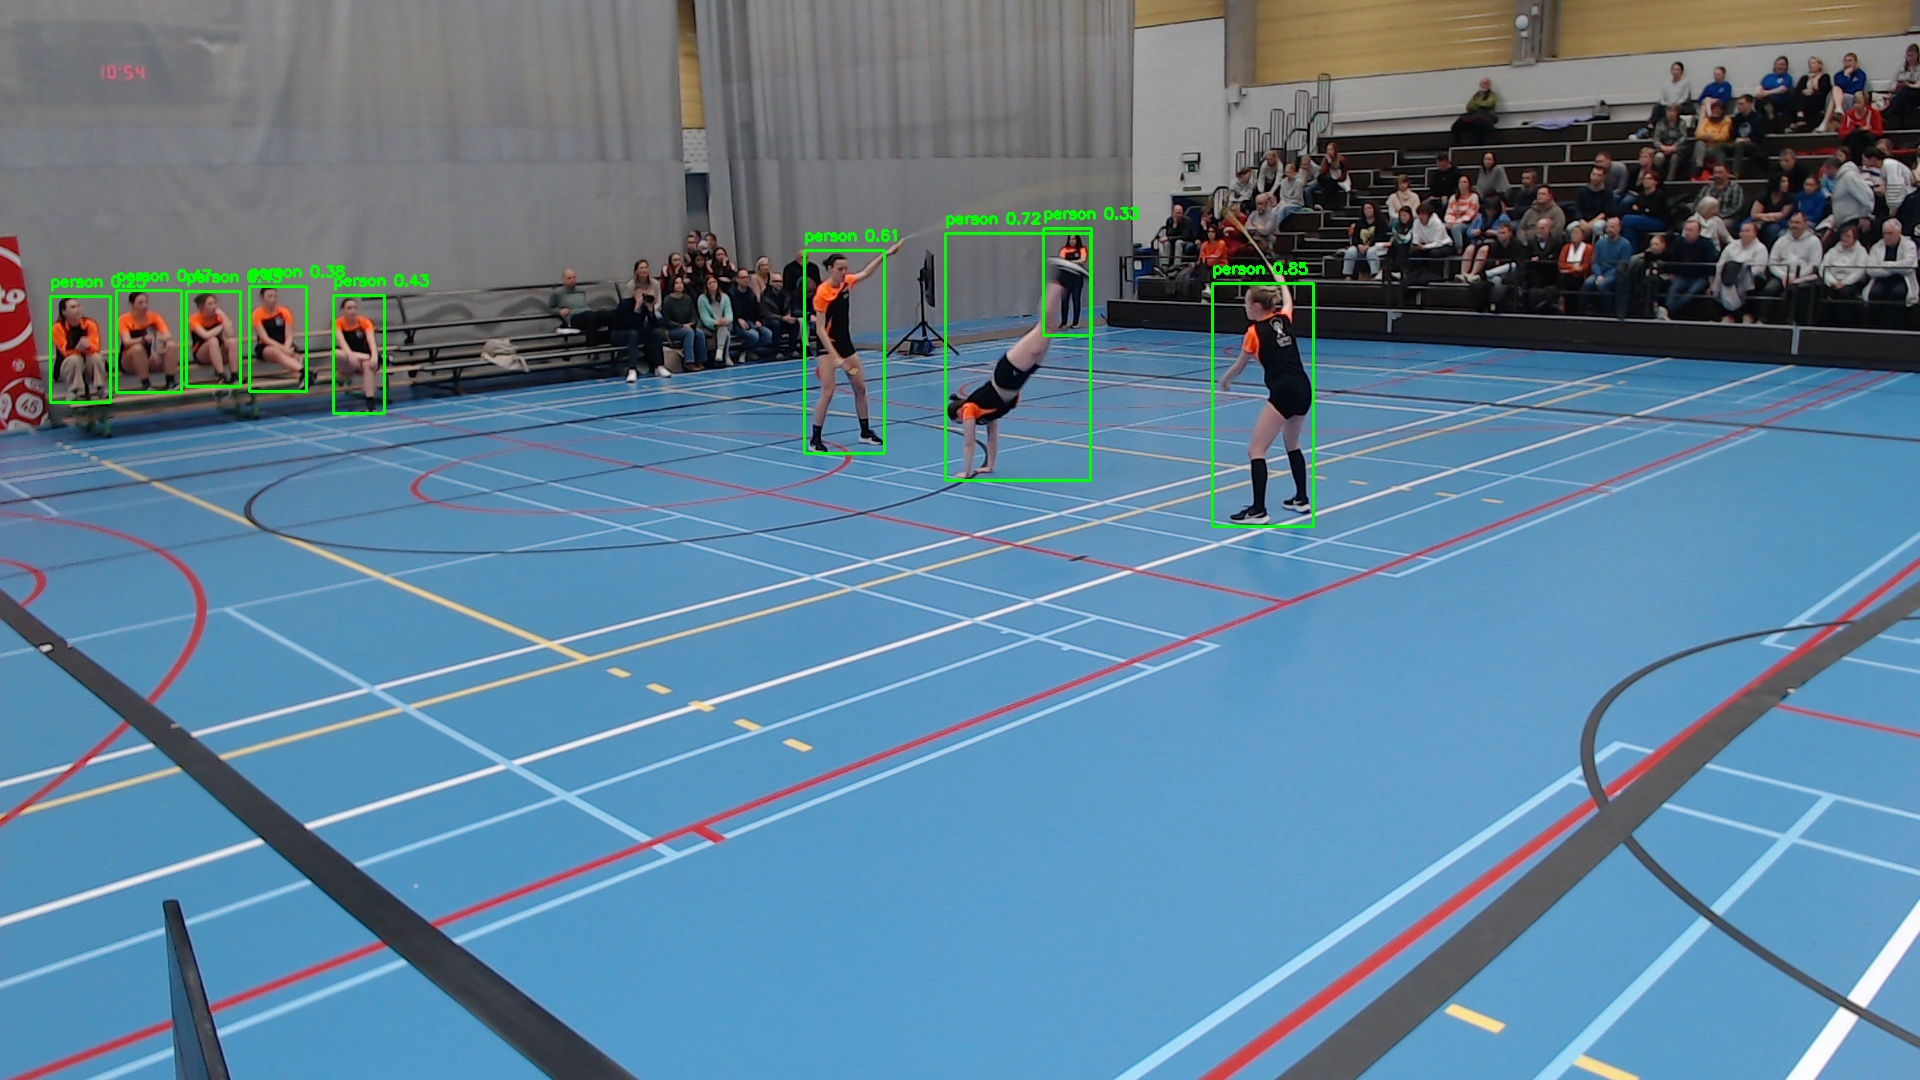
\includegraphics[width=0.95\linewidth]{img/1267_292_boxes}
    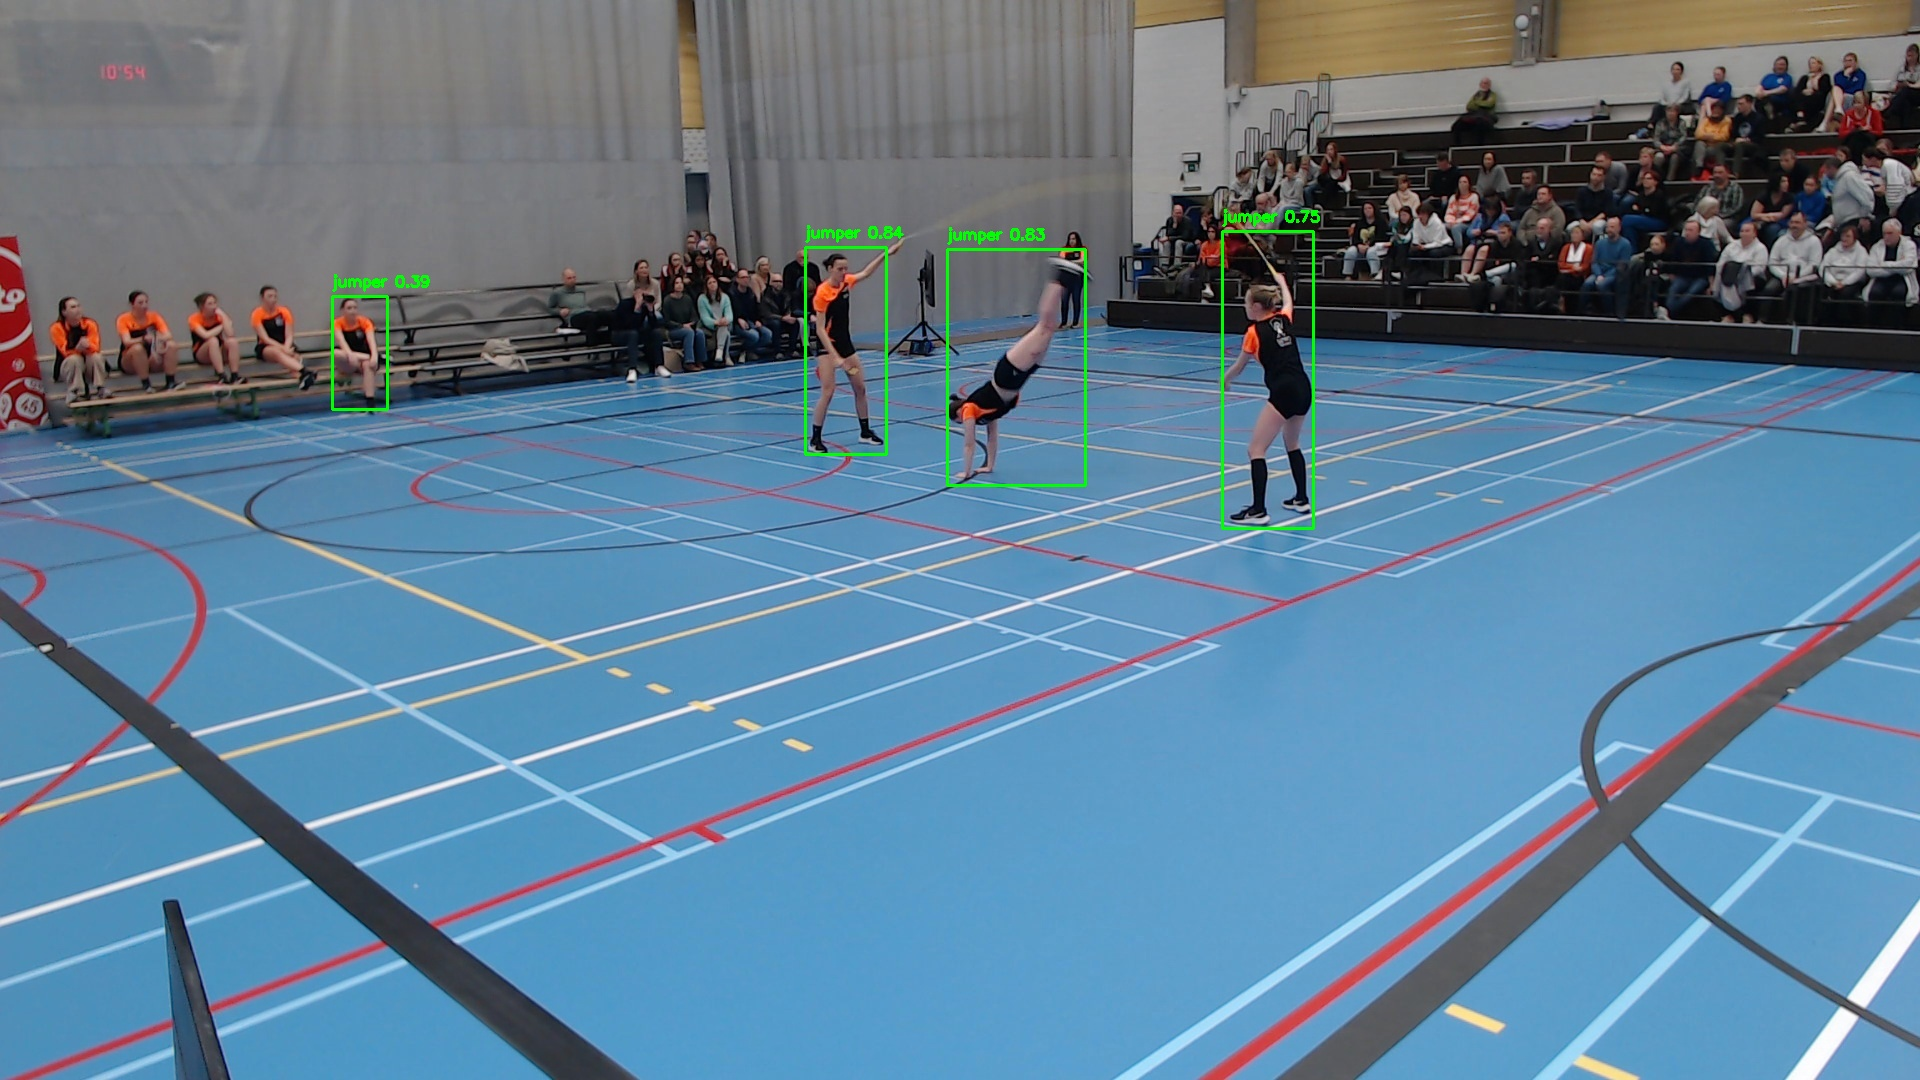
\includegraphics[width=0.95\linewidth]{img/1267_292_boxes_reduced_spectators}
    \caption[raw vs fine-tuned YOLOv11 nano model predictions]{Raw predictions of the unrefined YOLOv11 nano model compared to the fine-tuned model which reduces predictions of spectators.}
    \label{fig:raw-vs-fine-tuned-boxes}
\end{figure}

\begin{figure}
    \centering
%%    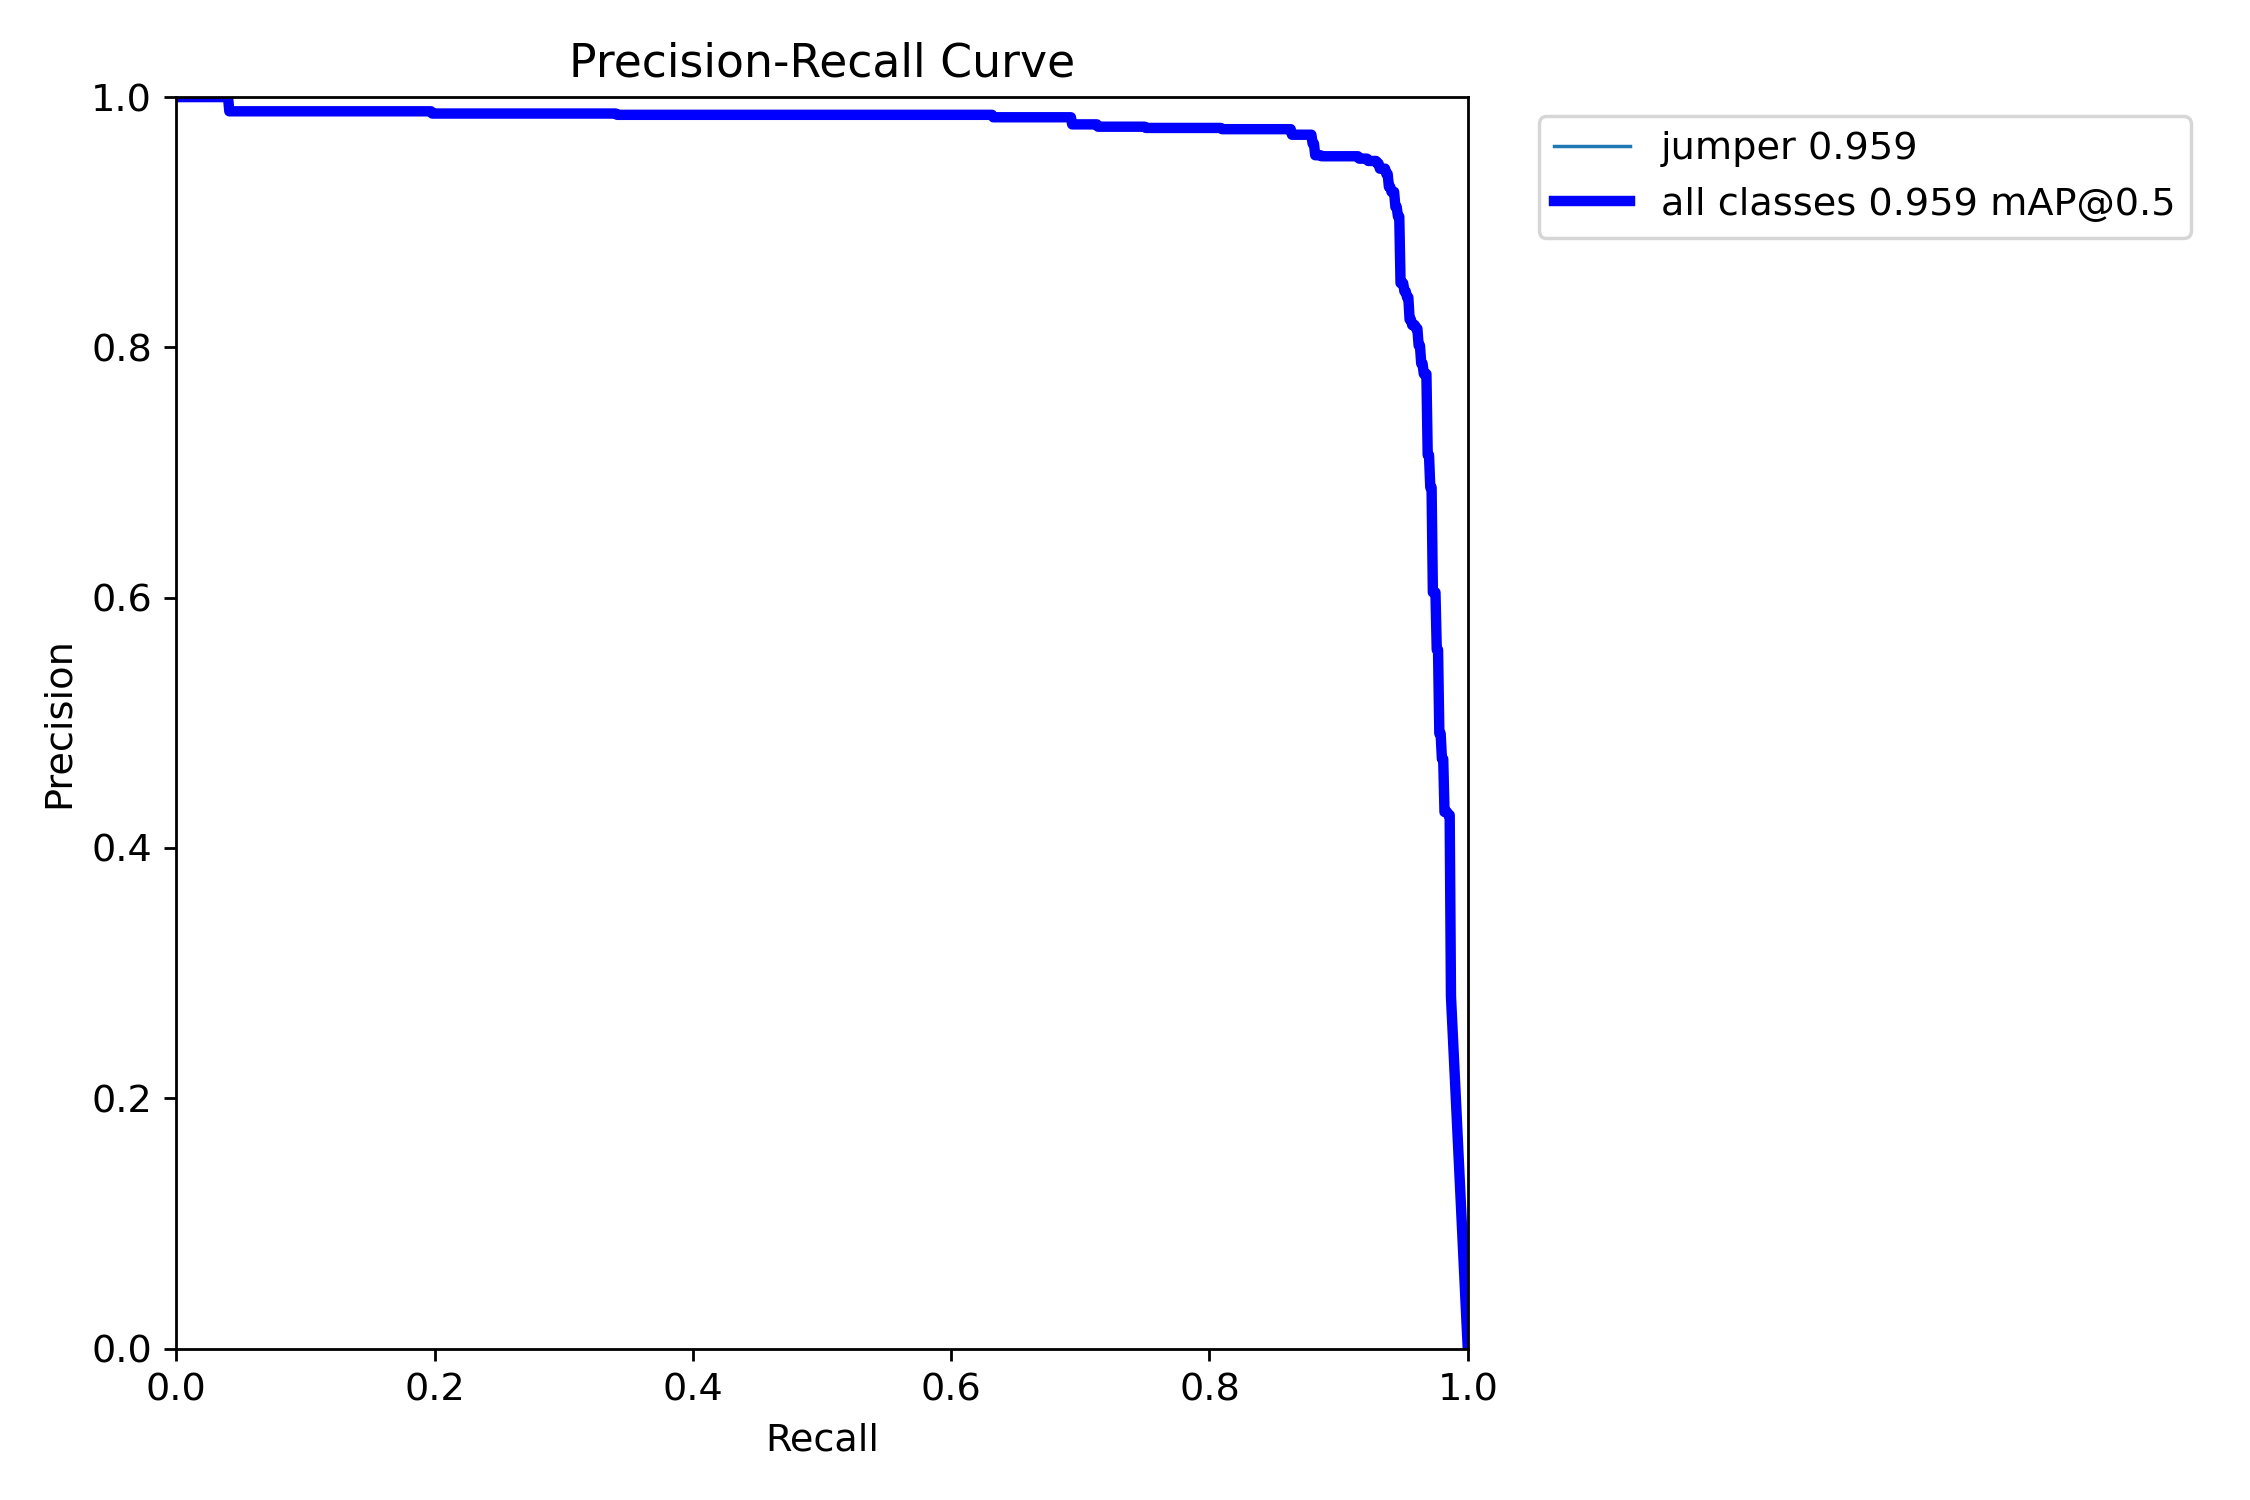
\includegraphics[width=0.35\linewidth]{img/PR_curve}
    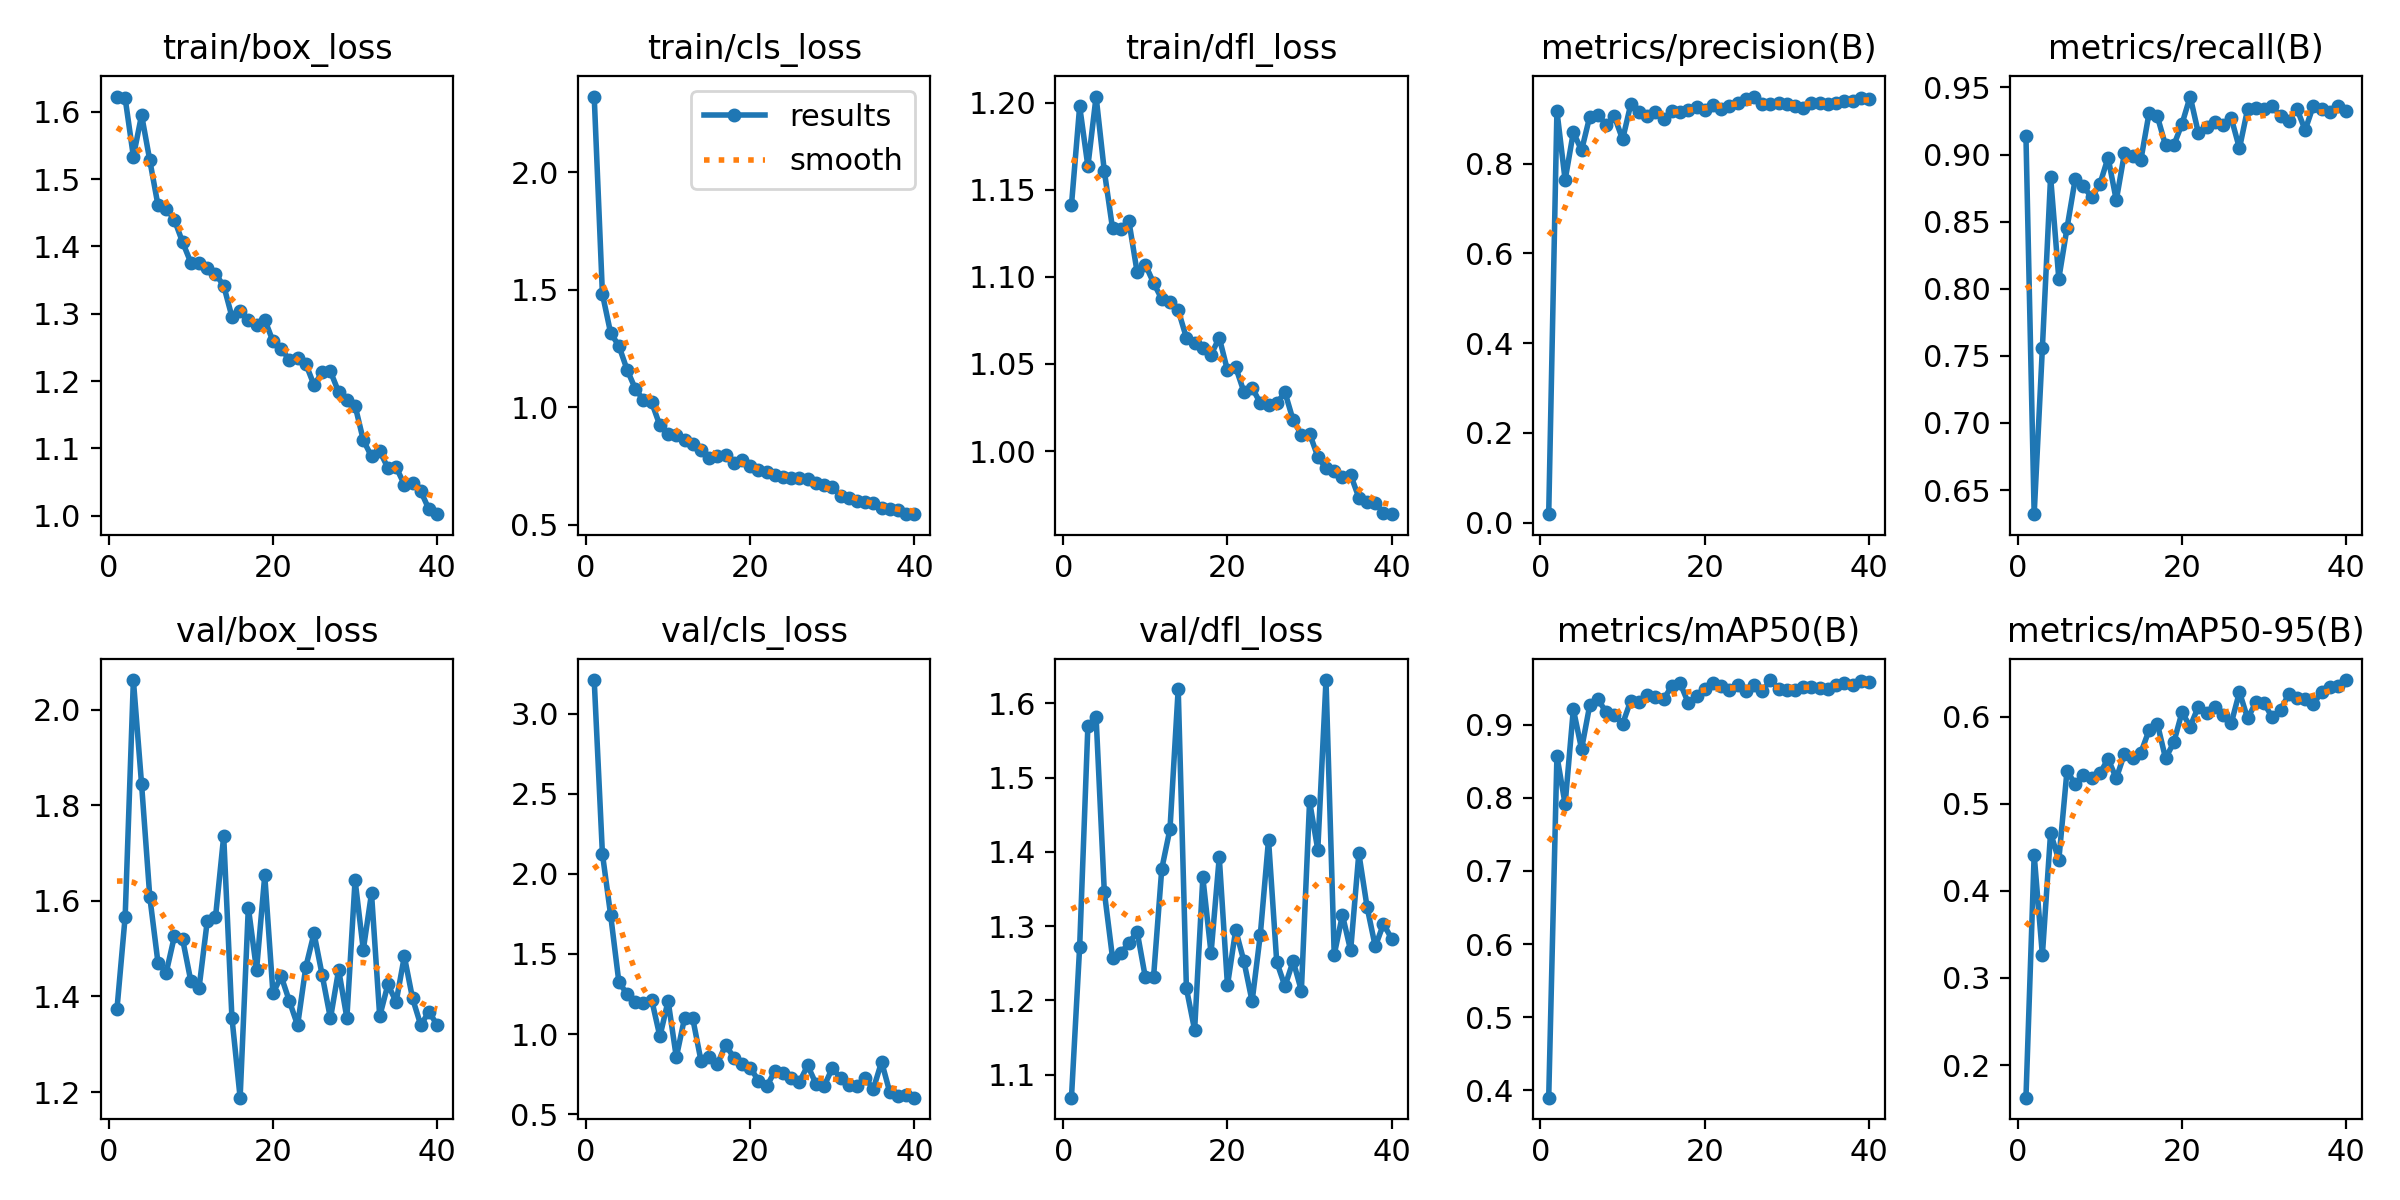
\includegraphics[width=0.95\linewidth]{img/results}
    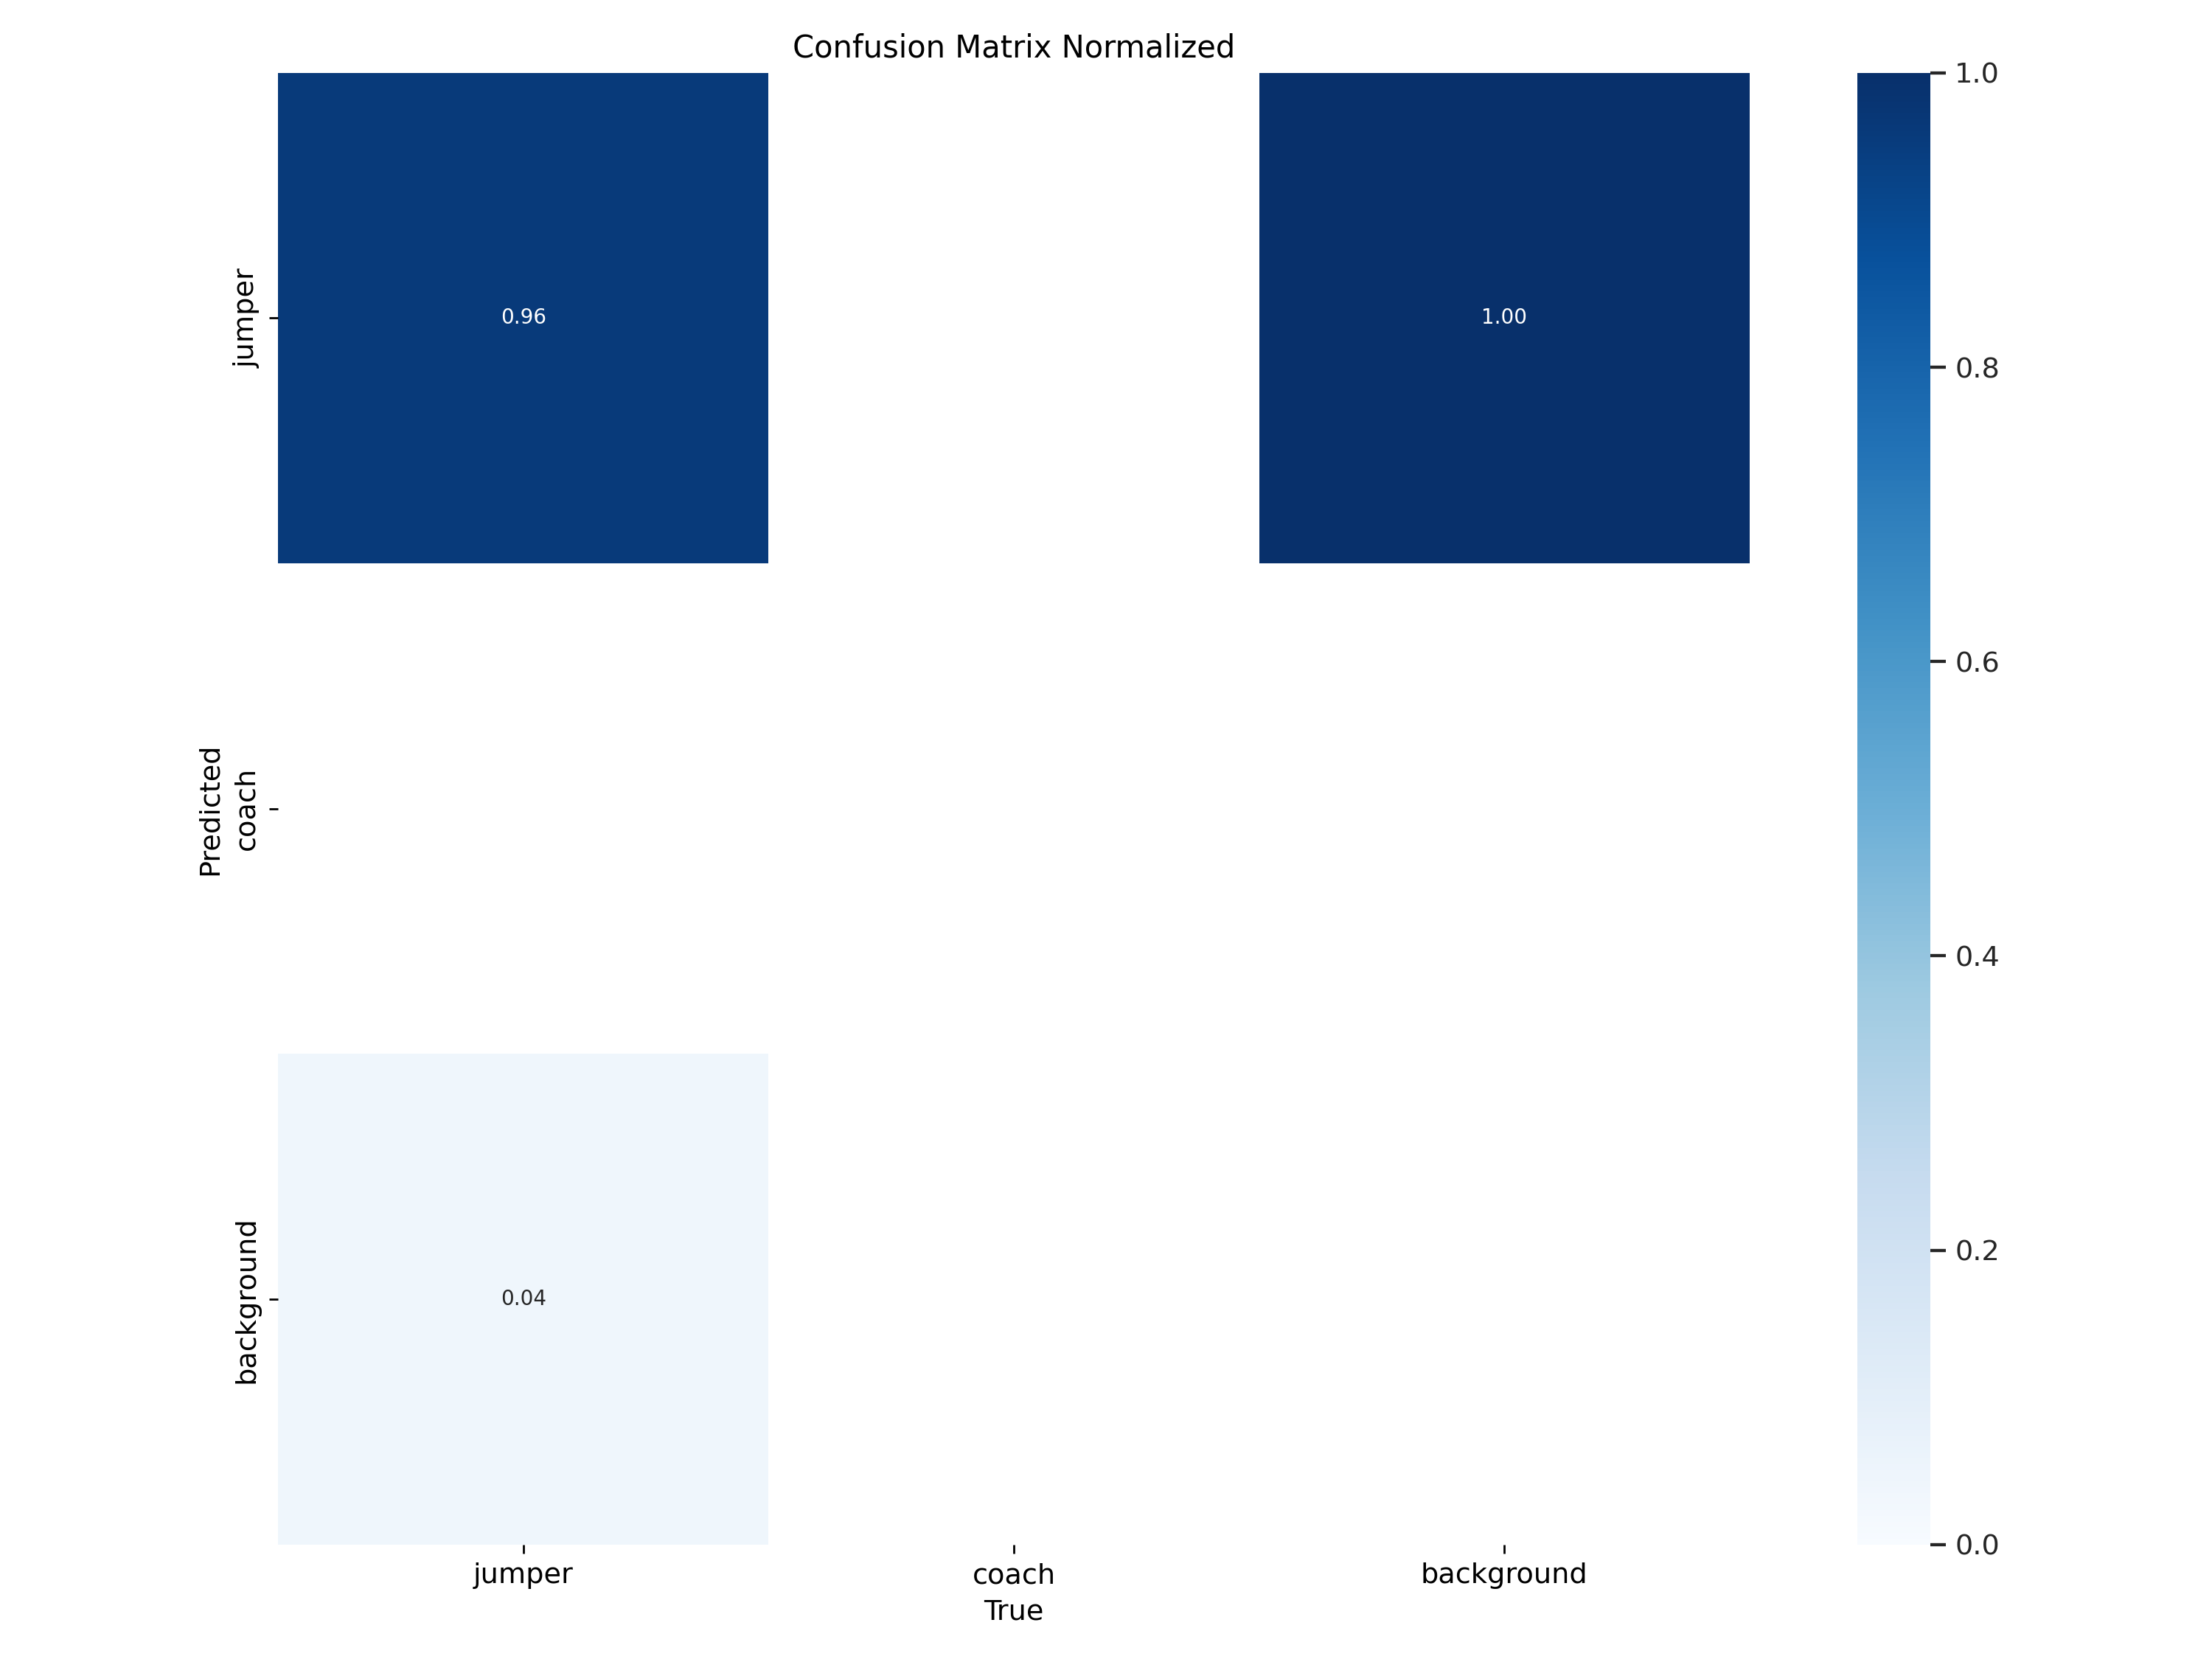
\includegraphics[width=0.85\linewidth]{img/confusion_matrix_normalized}
    \caption[metrics after fine-tuning YOLOv11]{Metrics after fine-tuning YOLOv11 on the validation set of 161 images, mAP50 of 0.953 \& mAP50-95 of 0.63, annotation of coaches was an idea.}
    \label{fig:localization-results}
\end{figure}

\begin{figure}
    \centering
    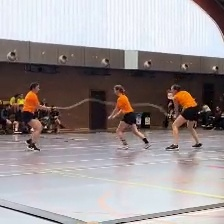
\includegraphics[width=0.45\linewidth]{img/1315_2935}
    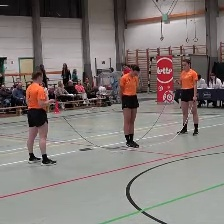
\includegraphics[width=0.45\linewidth]{img/2297_134}
    \caption[Valid crops of a DD3 routine on competition.]{Valid crops of a DD3 routine on competition.}
    \label{fig:dd3-crop}
\end{figure}

\begin{figure}
    \centering
    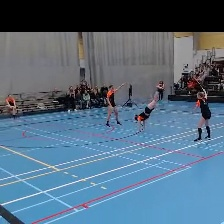
\includegraphics[width=0.45\linewidth]{img/1267_292_cropped}
    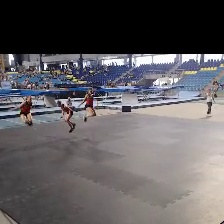
\includegraphics[width=0.45\linewidth]{img/1405_1061_cropped}
    \caption[dd3-crop-error]{Two crops were a spectator alongside the athletes.}
    \label{fig:dd3-crop-error}
\end{figure}

Annotating only athletes on 732 images \& fine-tuning the pre-trained nano yolo model, the first predictions of spectators are reduced considerately.
This way crops can be created by taking the minimum and maximum \(x\) \& \(y\)-coordinates. Reviewing cropped videos show indicate occasional frames predicting spectators, coaches or judges and moments of instability, as if you are watching camera footage of an earthquake.

In order to avoid a sudden zoom out, because of spectators, an IoU comparison of the previous predicted box with the new box is made. If the IoU value is larger than the average IoU of the last \(N\) seconds, powered to the fourth, than crop coordinates will be updated. Using the IoU comparison, reduces video crops including spectators, maintaining the earthquake effect.


To reduce shakiness and maintain a nice to watch cropped video, box-coordinates are smoothed out adapting box predictions of previous frames with the current one. This way, drastic changes in a predicted location, e.g. model ererrorror, arm or field movements aren't that drastic. Adaptation is done by incorporating two smooth values, indicating how much weight you give to the smoothed prediction of the previous frame. \footnote{Smoothed values are obtained by playing around with values, choosing those leading to the best, subjective, smoothed review}

$$ smth = smootval = 0.86  \quad \& \quad smths = smootval\_shrink = 0.94 $$

Which makes the new coordinates:

\begin{math}
   smooted_{x1_{min}} =
   \begin{cases}
       smooted_{x1_{min}} & \text{if} \quad iou < iou_{threshold} \\
       smth * smooted_{x1_{min}} + (1-smth) * x1_{min} & \text{else if} \quad x1_{min} < smooted_{x1_{min}} \\
       smths^ * smooted_{x1_{min}} + (1-smths) * x1_{min} & \text{otherwise}
   \end{cases}
\end{math}

The same is done for \( y1_{min}, x2_{max}, y2_{max} \).

Utilizing these steps allows for videos where a team is always on display (\ref{fig:dd3-crop}), with some videos still predicting spectators (\ref{fig:dd3-crop-error}) and a newly introduced problem, namely skippers running out of view.

% TODO : add movement corrector

\begin{figure}
    \centering
    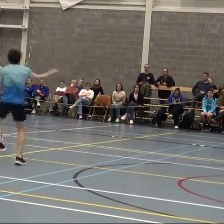
\includegraphics[width=0.45\linewidth]{img/1241_1093_cropped}
    \caption[dd3-crop-error]{Athletes running out of view.}
    \label{fig:dd3-crop-error-out-of-view}
\end{figure}

One way to solve jumpers running out of view, is by adding a default movement corrector, like the smooth value, which follows the new coordinates every frame. The movement corrector is based on the \(iou\)-value powered to the \(1/8\). It makes the crop following predictions by default, when IoU is getting low.


\begin{math}
    SQRT = 8 \\
    movementCorrector = iou^{1/SQRT} \\
    smooted_{x1_{min}} = smooted_{x1_{min}} * movementCorrector + (1 - movementCorrector) * {x1_{min}}
\end{math}



A possible improvement could be matching individual boxes with the new predictions, eliminating the spectator. Which raises concerns about jumpers entering the competition field. There are no earlier predicted boxes to match.
The total algorithm isn't perfect yet, but the results indicate sufficient valid video crops to use and experiment on segmentation and recognition.

\begin{listing}
    \begin{minted}{python}
        print('TODO : cleanup code')
    \end{minted}
    \caption[Example codefragment]{Example of adding cropping code.}
    \label{code:localization}
\end{listing}

Full code is visible in code snippet \ref{code:localization}. The results are broken down in table \ref{tbl:crop-results}.

% TODO: pairwise distances?

\begin{table}[h!]
    \begin{tabular}{|l|l|l|}
        \hline
        \textbf{videoId} & \textbf{seconds} & \textbf{reason} \\
        \hline
        \dots & \cellcolor{green!25} \dots & (other videos) \\ \hline
        1435 &	\cellcolor{green!25} 0 &	 \\ \hline
        1445 &	\cellcolor{green!25} 0 &	 \\ \hline
        2285 &	\cellcolor{green!25} 0 &	 \\ \hline
        2295 &	\cellcolor{green!25} 0 &	 \\ \hline
        2305 &	\cellcolor{green!25} 0 &	 \\ \hline
        2315 &	\cellcolor{green!25} 0 &	 \\ \hline
        995  &	\cellcolor{yellow!25} 5 &	Schocks \& turner out-of-view \\ \hline
        1275 &	\cellcolor{yellow!25} 1 &	aerial half \\ \hline
        1405 &	\cellcolor{orange!25} 30 &	spectator \\ \hline
        651  &	\cellcolor{yellow!25} 1    &	turner out of view \\ \hline
        664  &	\cellcolor{yellow!25} 1.5  &	turner out of view \\ \hline
        1202 &	\cellcolor{yellow!25} 5    &	turner out of view, recording itself \\ \hline
        1178 &	\cellcolor{yellow!25} 2    &	turner out of view \\ \hline
        1238 &	\cellcolor{yellow!25} 2    &	spectator before start routine \\ \hline
        1244 &	\cellcolor{yellow!25} 0    &	stopped following, remained in view \\ \hline
        1257 &	\cellcolor{yellow!25} 0    &	stopped following, remained in view \\ \hline
        1275 &	\cellcolor{yellow!25} 1.5  &	half out of view \\ \hline
        1339 &	\cellcolor{yellow!25} 8    &  spectator \\ \hline
        1444 &	\cellcolor{yellow!25} 1.5  &	half out of view \\ \hline
        2282 &	\cellcolor{yellow!25} 1    &	1 turner out of view, actual 3 sec no follow \\ \hline
        2317 &	\cellcolor{yellow!25} 2    &	minor shocks \\ \hline
        663  &	\cellcolor{orange!25} 25   &	Out-of-view \& shocks \\ \hline
        1241 &	\cellcolor{orange!25} 8    &	Out-of-view \\ \hline
        1267 &	\cellcolor{orange!25} 46   &	spectator \\ \hline
        1271 &	\cellcolor{orange!25} 24   &	Out-of-view \\ \hline
        1273 &	\cellcolor{orange!25} 8    &	Out-of-view \\ \hline
        1326 &	\cellcolor{orange!25} 6.5  &	spectator \\ \hline
        \(avg\) &	1.33 &	(seconds / 1m15) \\ \hline
        \(avg_{if}\) &	8.55 &	(seconds / 1m15) \\ \hline
        Nr of videos not ok &	21	& 15.6\% \\ \hline
        Total checked videos &	135	& (includes train videos) \\ \hline
    \end{tabular}
    \caption{Crop results manually checked. \\
    Yellow indicated videos are not disturbing for recognition, even though the crops aren't perfect. Orange videos require more attention and shouldn't be used for recognition. \\
    The \(avg_{if}\) indicates the average time in case a video has crops which aren't good.}
    \label{tbl:crop-results}
\end{table}









\section{Action segmentation}

Experiments on action segmentation have waited on skill recognition (section \ref{results:recognition}), this is why the experiments with action segmentation use the same models as the skill recognition, adapting only the top layers of the models.

To annotate which moments are interesting split points, the start and end frame of a skill receive value 1, while other frames remain 0.
As the start and end frame of a skill are rather subjective, frames around a split point also range somewhere in the interval \(]0, 1[\). These values are calculated using the function \ref{code:calculate-splitpoint-values} which is called on in the data generator demonstrated in code \ref{code:call-splitpoint-calculation}.
Each frame than has a value from zero to one. An example of consecutive splitpointvalues could be:

\([0, 0, 0.1, 0.31, 0.55, 0.86, 1, 0.86, 0.55, 0.31, 0.1, 0]\)

\begin{listing}
    \begin{minted}{python}
        def calculate_splitpoint_values(videoId: int, frameLength:int, df_Skills:pd.DataFrame, fps:float, Nsec_frames_around=1/6):
        """Creates a dataframe: 'videoId', 'frameNr', 'splitpoint'
        Where splitpoint is the value 0 -> 1 whether the video needs to be split at that point or not"""
        splitpoint_values = {
            'videoId' : [videoId for _ in range(frameLength)],
            'frameNr' : range(frameLength),
            'splitpoint' : [0 for _ in range(frameLength)],
        }

        frames_around_splitpoint = round(Nsec_frames_around * fps)
        for _, skillrow in df_Skills.iterrows():
            frameStart = skillrow["frameStart"]
            frameEnd = skillrow["frameEnd"]

            currentFrameStart = frameStart - frames_around_splitpoint
            currentFrameEnd = frameEnd - frames_around_splitpoint
            while currentFrameStart < frameStart + frames_around_splitpoint:
                framesApart = abs(currentFrameStart - frameStart)
                splitvalue = 1 - (framesApart/frames_around_splitpoint) ** 2
                splitvalue *= splitvalue

                currentFrameStart += 1
                currentFrameEnd += 1

                splitpoint_values['splitpoint'][currentFrameStart] = splitvalue
                if currentFrameEnd < frameLength:
                    splitpoint_values['splitpoint'][currentFrameEnd] = splitvalue

        return pd.DataFrame(splitpoint_values)
    \end{minted}
    \caption[call-splitpoint-calculation]{call-splitpoint-calculation}
    \label{code:calculate-splitpoint-values}
\end{listing}


\begin{listing}
    \begin{minted}{python}
        df = calculate_splitpoint_values(
            videoId=videoId,
            frameLength=frameLength,
            df_Skills=self.Skills[self.Skills['videoId'] == videoId],
            fps = row["fps"]
        )
    \end{minted}
    \caption[call-splitpoint-calculation]{call-splitpoint-calculation}
    \label{code:call-splitpoint-calculation}
\end{listing}


\subsection{Video Vision Transformer \& Self-attention ConvLSTM}

The first and second experiment for segmention use code implementations of the video vision transformer as described in \textcite{Arnab2021} and the Self-Attention ConvLSTM from \textcite{Lin_2020}.
Implementations of these models, ViViT \ref{code:get_model_ViViT} and SA-ConvLSTM (TODO), are aided by \textcite{OpenAI_ChatGPT_2025} and \textcite{Deepseek_2025}.
These models were then trained on 7.8k batches of 16 consecutive frames, which originate from 44 trainings videos for about 48 minutes of training data, having framerates between 25 and 60 \footnote{Most labeled videos have a framerate of 25, 30 or 50 frames per second}.
Both models showed the same results, averaging out predictions slightly above 0 for all frames, stagnating on MSE losses of around 0.09 and 0.10. (Exact values are lost due to the switch to pytorch and bugs, will be re-added later.)

\begin{listing}
    \begin{minted}{python}
        import keras
        import pandas as pd
        import tensorflow as tf
        import numpy as np
        import matplotlib.pyplot as plt
        import sys
        sys.path.append('..')
        from api.helpers import ConfigHelper
    \end{minted}
    \caption[imports-ViViT]{imports-ViViT}
    \label{code:imports-ViViT}
\end{listing}


\begin{listing}
    \begin{minted}{python}
        def mlp(x, hidden_units, dropout_rate):
            for units in hidden_units:
                x = keras.layers.Dense(units, activation=keras.activations.gelu)(x)
                x = keras.layers.Dropout(dropout_rate)(x)
            return x
    \end{minted}
    \caption[mlp layer]{ViViT: multi-layer-perceptron}
    \label{code:mlp-layer}
\end{listing}


\begin{listing}
    \begin{minted}{python}
    def __init__(self, patch_size):
        super().__init__()
        self.patch_size = patch_size

    def call(self, images):
        input_shape = keras.ops.shape(images)
        batch_size = input_shape[0]
        timestep = input_shape[1]
        height = input_shape[2]
        width = input_shape[3]
        channels = input_shape[4]
        num_patches_h = height // self.patch_size
        num_patches_w = width // self.patch_size

        def create_single_timepatch(video_input):
            patches = keras.ops.image.extract_patches(video_input, size=self.patch_size)
            patches = keras.ops.reshape(
                patches,
                (
                    num_patches_h * num_patches_w * timestep,
                    self.patch_size * self.patch_size * channels,
                ),
            )

            return patches

        patches = tf.map_fn(create_single_timepatch, images)

        return patches

    \end{minted}
    \caption[time-patches]{ViViT: Time Patches}
    \label{code:timepatches}
\end{listing}


\begin{listing}
    \begin{minted}{python}
        def get_model(modelinfo):
            inputs = keras.Input(shape = (modelinfo['timesteps'], modelinfo['dim'], modelinfo['dim'], 3))
            patches = TimePatches(modelinfo['patch_size'])(inputs)
            num_patches = (modelinfo['dim'] // modelinfo['patch_size']) ** 2
            encoded_patches = TimePatchEncoder(num_patches, modelinfo['timesteps'], modelinfo['dim_embedding'])(patches)
            print("shape of encoded_patches", encoded_patches.shape)

            # Create multiple layers of the Transformer block.
            for _ in range(modelinfo['encoder_blocks']):
                # Layer normalization 1.
                x1 = keras.layers.LayerNormalization(epsilon=1e-6)(encoded_patches)
                attention_output = keras.layers.MultiHeadAttention(
                num_heads=modelinfo['num_heads'], key_dim=modelinfo['dim_embedding'], dropout=0.1
                )(x1, x1)
                # Skip connection 1.
                x2 = keras.layers.Add()([attention_output, encoded_patches])
                # Layer normalization 2.
                x3 = keras.layers.LayerNormalization(epsilon=1e-6)(x2)
                x3 = mlp(x3, hidden_units=[modelinfo['dim_embedding'] ** 2, modelinfo['dim_embedding']], dropout_rate=0.1)
                # Skip connection 2.
                encoded_patches = keras.layers.Add()([x3, x2])

            # Create a [batch_size, projection_dim] tensor.
            representation = keras.layers.LayerNormalization(epsilon=1e-6)(encoded_patches)
            representation = keras.layers.Flatten()(representation)
            representation = keras.layers.Dropout(0.3)(representation)

            features = mlp(representation, hidden_units=modelinfo['mlp_head_units'], dropout_rate=0.3)

            ...

    \end{minted}
    \caption[get model ViViT]{ViViT: get model ViViT (keras), without output layer (part 1)
    (Possible bugfixes done using \textcite{OpenAI_ChatGPT_2025})}
    \label{code:get_model_ViViT}
\end{listing}

\begin{listing}
    \begin{minted}{python}
        # ... (this is the output layer of segmentation)
        classes = modelinfo['timesteps']
        outputs = keras.layers.Dense(classes, activation='softmax')(features)

        return keras.Model(inputs=inputs, outputs=outputs)
    \end{minted}
    \caption[ViViT output segmentation]{ViViT output segmentation using features of code fragment \ref{code:get_model_ViViT}}
    \label{code:ViViT-output-segmentation}
\end{listing}


\subsection{pre-trained MViT}

In order to get better results on the little labeled available data, (44 videos for training, 7 validation videos), looking for a pre-trained model really helped a lot.
PyTorch provides a \href{https://pytorch.org/vision/main/models.html}{list} of pre-build and pre-trained models such as \href{https://pytorch.org/vision/main/models/video_mvit.html}{mvit-v1-b}.
Fine-tuning this model lowered the MSE to 0.065 with peaks overlapping splitpoints as demonstrated and elaborated in figure \ref{fig:segmentation-plot}.

To get al sections, all peaks in its neighborhood (\(windowsize = fps / 3\)) having a splitpoint value more than 0.4 become the start and end frame of a skill section, which will be used to recognize which skill is displayed. The code filtering segments out of raw-predicted splitpoint values, as used in the segmentation-plot \ref{fig:segmentation-plot} can be found in code snippet \ref{code:predictions-to-splitpoints}.

\begin{listing}
    \begin{minted}{python}
        predictions = np.array(predictions)
        predictions_bigger_than_split_threshold = np.where(predictions > split_threshold, predictions, 0)
        p_split = predictions_bigger_than_split_threshold
        window_size = int(fps // 3)
        predictions_argMax_in_window = [s - window_size + np.argmax(p_split[max(0, s-window_size):min(frameLength, s+window_size)]) for s in range(frameLength)]
        predictions_splitmoments = np.where(predictions > split_threshold, predictions_argMax_in_window, 0)
        predictions_splitmoments = np.unique(predictions_splitmoments)

        distances = predictions_splitmoments[1:] - predictions_splitmoments[:-1]
        predictions_splitmoments = predictions_splitmoments[1:]
        predictions_splitmoments = predictions_splitmoments[np.where(distances < window_size // 3, False, True)]
        predictions_splitmoments = [int(g) for g in predictions_splitmoments]
    \end{minted}
    \caption[predictions-to-splitpoints]{Code which filters splitpoints from the raw predicted splitpoint values to frame numbers.}
    \label{code:predictions-to-splitpoints}
\end{listing}


\begin{figure}
    \centering
    \includegraphics[width=0.45\linewidth]{img/segmentplot_2285_frameStart_2250_with_250_points}
    \includegraphics[width=0.45\linewidth]{img/segmentplot_2285_frameStart_2500_with_250_points}    \includegraphics[width=0.45\linewidth]{img/segmentplot_2285_frameStart_2750_with_250_points}    \includegraphics[width=0.45\linewidth]{img/segmentplot_2285_frameStart_3000_with_250_points}
    \caption[Segmentation plot]{Segmentation plot comparing predictions with the splitpoint values indicating a match of interesting splitpoint. Visible errors are: \\
        at frame 2459, a relatively lower jump out of the rope with a snapper. \\
        at frames 2700 until 2900 indicating a transition which is labeled in one segment, but the athletes are rather bouncy on their feet, letting the model think those are splitpoints.
        a handspring occurs from frame 3140 until 3192, but the model indicates to much during the skill, while it doesn't indicate the moment right after the handspring.
    }
    \label{fig:segmentation-plot}
\end{figure}

(Ideas for additional metrics such as avg distance between nearest peak and splitpoint, IoU like overlap with nearest peaks will follow later \& further research on segmentation will follow in another submit.)

These predicted segments are the first usable split moments to use for splitting unseen videos recognizing or speeding up further labeling.

\section{Skill recognition}
\label{results:recognition}

The first trials from scratch, a video vision transformer, which is adapted from the transformer created during classes. Adding the convolution layer in front and the time dimension created the ViViT transformer as proposed in (source).
Idea's add extra convolution layers \& use pre-trained model.

Elaborate 16 frame time aspect.

\subsection{Video Vision Transformer}

For training the video vision transformer, the data is upsampeled

\subsection{Multiscale Video Vision Transformer - MViT}
\href{https://pytorch.org/vision/main/models/video_mvit.html}{Pytorch MViT}

Pytorch implementation of source.

For the first training round a double upgrade has been performed. The first adaption is downsampling the skills in 5 main classes to predict.  \& pre-trained model.

\begin{table}[h!]
    \centering
    \begin{tabular}{|r|r|l|r|r|}
        \hline
        \textbf{Train \%} & \textbf{Train Count} & \textbf{Skill} & \textbf{Val Count} & \textbf{Val \%} \\
        \hline
        50.6687 & 2273 & jump & 379 & 56.6517 \\
        14.0660 & 631 & pushup & 77 & 11.5097 \\
        13.0629 & 586 & return from power & 84 & 12.5561 \\
        9.8529 & 442 & frog & 59 & 8.8191 \\
        3.2100 & 144 & crab & 9 & 1.3453 \\
        2.0062 & 90 & split & 12 & 1.7937 \\
        1.1146 & 50 & flip & 5 & 0.7474 \\
        0.9140 & 41 & rondat & 5 & 0.7474 \\
        0.8917 & 40 & rad & 3 & 0.4484 \\
        0.8025 & 36 & suicide & 8 & 1.1958 \\
        0.7356 & 33 & handspring & 5 & 0.7474 \\
        0.6910 & 31 & rol2kip & 7 & 1.0463 \\
        0.4458 & 20 & kip & 6 & 0.8969 \\
        0.3567 & 16 & speed & NULL & NULL \\
        0.3121 & 14 & kopkip & 1 & 0.1495 \\
        0.2675 & 12 & roll & 3 & 0.4484 \\
        0.1783 & 8 & stut & 2 & 0.2990 \\
        0.1337 & 6 & swift & NULL & NULL \\
        0.1337 & 6 & UNKOWN & 1 & 0.1495 \\
        0.0669 & 3 & leapfrog & NULL & NULL \\
        0.0446 & 2 & footwork-kick & NULL & NULL \\
        0.0223 & 1 & mountainclimber & NULL & NULL \\
        0.0223 & 1 & footwork-open & 1 & 0.1495 \\
        \hline
    \end{tabular}
    \caption{Skill distribution with training and validation counts and percentages. Null values indicate missing validation data.}
    \label{tab:skill_distribution_full_with_nulls}
\end{table}


\begin{table}[h!]
    \centering
    \begin{tabular}{|l|r|r|r|r|}
        \hline
        \textbf{Skill} & \textbf{Train Count} & \textbf{Train \%} & \textbf{Val Count} & \textbf{Val \%} \\
        \hline
        jump & 2273 & 50.6687 & 379 & 56.6517 \\
        pushup & 631 & 14.0660 & 77 & 11.5097 \\
        return from power & 586 & 13.0629 & 84 & 12.5561 \\
        frog & 442 & 9.8529 & 59 & 8.8191 \\
        other & 526 & 11.7253 & 68 & 10.1645 \\
        \hline
    \end{tabular}
    \caption{Train and validation skill distribution with low-frequency skills grouped as "other"}
    \label{tab:skill_distribution_grouped_final}
\end{table}


\section{Model verification}

Comming soon... (Mapping predicted skills, turners, rotations... to its perspective level which will be compared with the score assigned by judges on competition.)

\begin{listing}
    \begin{minted}{python}
        print('TODO : cleanup code')
    \end{minted}
    \caption[]{}
    \label{code:}
\end{listing}

\begin{listing}
    \begin{minted}{python}
        print('TODO : cleanup code')
    \end{minted}
    \caption[]{}
    \label{code:}
\end{listing}

\begin{listing}
    \begin{minted}{python}
        print('TODO : cleanup code')
    \end{minted}
    \caption[]{}
    \label{code:}
\end{listing}